\section{基于邻域的分类}
\label{sec:classification-instances}

前面的线性分类器用一组全局权重决定边界。如果同一类别分布在几个相隔的区域，一条直线可能无法把它们同时与另一类分开。我们也可以暂不规定整条边界的形状，而在新输入附近寻找带标签的样本，用这些局部记录判断类别。这是$k$-NN分类的做法：保存训练实例，按距离找出邻居，再聚合标签。与回归中的响应平均相比，分类采用多数投票或局部类别比例。近邻表示和检索的基础见第\ref{sec:classic-overview-neighborhood}节，回归对应形式见第\ref{sec:regression-knn}节。

\subsection{$k$近邻分类（$k$-NN）}
\label{sec:classification-knn}

局部比较避开了预先选择全局边界，却留下一个问题：附近只取一个样本，还是让多个样本一起判断？最近的样本也可能带有噪声标签；增加邻居能平均这种波动，但范围过大又会把别处的类别混进来。近邻数因此决定了我们用多大范围的标签来描述当前输入。

Cover与Hart在1967年的论文中回顾了Fix与Hodges始于1951年报告的近邻判别研究：在所研究的条件下，让近邻数随样本量增长、同时让其占比趋于零，可以获得一致性。Cover与Hart则分析了始终只取一个最近邻时，极限错误率与贝叶斯风险之间的界。前者研究增长近邻数怎样平均标签噪声，后者刻画单个邻居仍保留多少判别信息\scite{coverhart1967}。

\subsubsection{模型结构}
\label{sec:classification-knn-structure}

给定训练集$D_n=\{(\bm{x}_i,y_i)\}_{i=1}^n$、距离$\rho$以及$1\leq k\leq n$，用$N_k(\bm{x})\subseteq\{1,\ldots,n\}$表示查询$\bm{x}$的$k$个最近邻索引。预测规则为
\begin{equation}
  \hat h_{n,k}(\bm{x})
  =\argmax_{c\in\{1,\ldots,C\}}
  \sum_{i\in N_k(\bm{x})}\mathbb{1}\{y_i=c\}.
  \label{eq:classification-knn-vote}
\end{equation}
距离相同时，按预先约定、独立于标签的顺序选取邻居；类别票数并列时也使用固定规则。多分类在奇数$k$时也可能出现票数并列，因此两种平局都需要明确规则。

式\eqref{eq:classification-knn-vote}也可以理解为估计查询附近的类别比例：
\begin{equation}
  \hat\eta_{n,c}(\bm{x})
  =\frac{1}{k}\sum_{i\in N_k(\bm{x})}\mathbb{1}\{y_i=c\},
  \qquad
  \hat h_{n,k}(\bm{x})=\argmax_c\hat\eta_{n,c}(\bm{x}).
  \label{eq:classification-knn-posterior}
\end{equation}
比例估计解释了投票为什么可能有效：若邻域内的条件类别分布变化不大，邻居标签就能提供关于当前输入的统计证据。局部比例的误差取决于邻域大小与标签噪声，概率质量需通过样本外数据检验。

图~\ref{fig:classification-knn-neighborhood}固定训练点和查询，只改变参与投票的近邻数。取查询$\bm{x}=(0,0)$，样本1、3、4、6属于类1，其余样本属于类2。按欧氏距离计算，七个样本到查询的平方距离依编号为$1,2,2.5,4.25,5,9,10.25$，因此编号也表示由近到远的次序。

$k=1$时只有样本1投票，查询被判为类1；$k=5$时样本1至5投票，其中类1有三票、类2有两票，预测仍为类1。两幅图中的圆分别经过第1和第5个邻居，半径为$1$和$\sqrt5$。圆表示当前查询的证据范围，整个平面上的分类边界则由各查询的投票共同决定。比较两个$k$的准确性还需要查询的真实标签。

\begin{figure}[htbp]
  \centering
  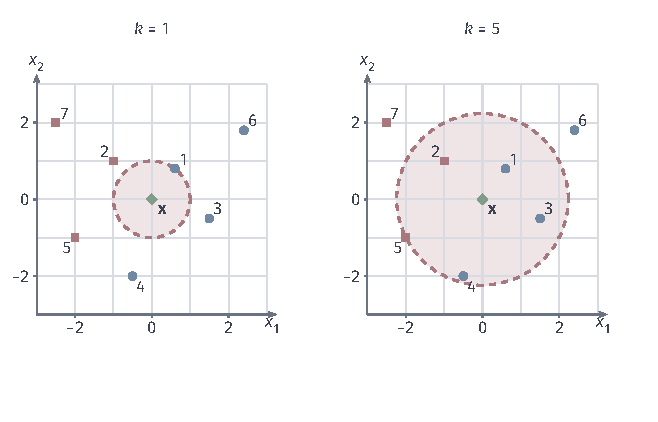
\includegraphics[width=111.404mm]{figures/04-classic-models/00-shared/tikz/classification-knn-neighborhood/figure.pdf}
  \caption{同一查询下的近邻范围与投票变化。教学构造取$n=7$、$d=2$、无量纲坐标和欧氏距离，查询为$\bm{x}=(0,0)$；两图的样本、编号及坐标尺度完全相同。蓝色圆点表示类1，红色方点表示类2，绿色菱形表示查询，红色虚线圆表示包含边界的近邻范围。左图$k=1$、半径$1$，蓝、红票数为$1:0$；右图$k=5$、半径$\sqrt5$，票数为$3:2$，因此判为蓝色类。各邻居等权投票，距离和票数均无并列；点的位置、标签与参数均为人为设定，不代表真实数据实验。}
  \label{fig:classification-knn-neighborhood}
\end{figure}

\subsubsection{参数学习}
\label{sec:classification-knn-learning}

基本$k$-NN分类没有固定维数参数的优化过程，但需要确定输入表示、距离、近邻数及检索方式。“非参数化”是指预测关系不局限于一个固定有限维参数族；它仍有超参数，预处理和模型选择也属于学习。

距离决定哪些样本会参与投票。对数值特征，欧氏距离$\rho(\bm{x},\bm{z})=\lVert\bm{x}-\bm{z}\rVert_2$容易计算，却会放大数值范围较大的坐标。收入和年龄共同作为特征时，直接使用原始单位会让收入差异主导距离。标准化、按业务意义设定尺度或学习特征权重都可改变这一点；不同特征的重要性可通过任务知识或训练数据确定。标准化参数只能从训练集估计，交叉验证时应在各训练折内重新拟合，避免验证信息提前进入距离。

类别型特征可采用\term{汉明距离}（Hamming distance），按不同取值的坐标数比较，而不能把任意类别编码的数字差当成有意义的远近。文本的TF--IDF等稀疏向量常比较余弦相似度，强调方向而非长度；$1$减余弦相似度一般不满足三角不等式，不能直接套用所有度量空间结论。对非零向量作单位长度归一化后，按余弦相似度排序与按欧氏距离排序等价，此时可用欧氏空间中的解释。

若特征之间相关，可以考虑\term{马氏距离}（Mahalanobis distance），用协方差调整方向上的尺度：
\begin{equation}
  \rho_{\mathrm{M}}(\bm{x},\bm{z})^2
  =(\bm{x}-\bm{z})^\top
   \bm{\Sigma}^{-1}(\bm{x}-\bm{z}),
  \label{eq:classification-mahalanobis}
\end{equation}
其中$\bm{\Sigma}\in\mathbb{R}^{d\times d}$须正定。样本不足时协方差估计可能奇异，需要正则化；整体协方差也不一定符合分类所需的相似性。

近邻数$k$控制局部平均的范围。$k=1$时，一个错误标签就会影响邻近查询；增加邻居可平均这类波动，也会混入更远区域并削弱局部细节。因此$k$的选择需要结合类别比例、局部密度与距离表示，在训练集内部验证。$k\approx\sqrt n$可以作为搜索起点，最终选择依据相同评价条件下的误差。

检索代价需要区分距离计算与邻居选择。对一个$d$维稠密查询，朴素扫描$n$个训练样本计算距离需$O(nd)$；若再把所有距离排序，总代价为$O(nd+n\log n)$。采用线性选择算法得到最小的$k$项，再作投票，可达$O(nd+n+k)$；使用大小为$k$的堆则需$O(nd+n\log(k+1)+k)$。因此，通常所说的$O(nd)$朴素预测复杂度隐含了无需完整排序的选择方法。训练集的存储为$O(nd)$，批量计算、硬件、精度要求和延迟预算共同决定这种实现的可用规模。

KD树或球树（ball tree）等精确索引通过空间划分排除不可能更近的样本。低维且分布有利时，它们可以减少访问量；最坏情形仍会检查大部分样本。索引保留原预测规则，选择时比较建索引成本、内存和实际查询时间，维数的影响需结合数据分布测量。

对高维大规模数据，还可以用\term{近似最近邻检索}（approximate nearest-neighbor search）交换少量检索误差与计算收益。局部敏感哈希（locality-sensitive hashing, LSH）让相近向量较可能进入同一哈希桶；分层可导航小世界图（hierarchical navigable small world, HNSW）沿多层邻接图逐步寻找候选；倒排文件与乘积量化（inverted file with product quantization, IVF--PQ）先缩小候选分区，再用压缩编码近似距离。这些方法的搜索预算和压缩程度会改变邻居集合，需同时检查邻居召回率与最终分类误差。以下理论以精确检索为前提，不直接覆盖任意近似索引。

\subsubsection{理论分析}
\label{sec:classification-knn-theory}

\paragraph{表达能力}
固定$n$、$k$及欧氏距离后，一个候选规则由$n$个锚点的位置与类别共同规定：查询时取最近的$k$个锚点，再按既定平局规则比较票数。考察所有可能的锚点位置与类别，才能说明这一规则族能够表达哪些目标。每个候选都是分段常值函数；邻居集合只在锚点的等距平面处改变，同一邻居集合给出相同票数。

锚点可以让一个类别占据几个分离的区域。例如，$k=1$时将四个锚点放在前面的异或输入$(\pm1,\pm1)$上，并赋予相应类别，坐标轴便把平面划成四个最近锚点区域；四个开象限的类别可全部吻合异或目标。更一般地，若各目标类别对应的输入集合都紧致，不同类别集合之间的距离至少为$\Delta>0$，可在每类选取有限个锚点，使该类每个输入到同类锚点的距离小于$\Delta/2$。当$n$足以容纳这一覆盖时，异类锚点至少相距$\Delta$，这组1-NN候选便能精确表示整个目标支持上的类别。

有限锚点仍限制了边界形状。在平面上按单位圆的内外区分类别时，有限条等距直线不能拼成整条圆周，任一有限锚点候选都无法处处吻合这个目标。若输入表示又把不同目标类别映到同一点，所有基于该表示的候选都会对它们给出相同判断。

票数比例还有独立于分区形状的限制。固定$k$时，每类比例只能取$0,1/k,\ldots,1$，不能精确表示任意后验概率。例如两类、$k=3$且真实正类后验恒为$3/10$时，任一候选在每个输入处的概率差都至少为$1/30$。增加锚点数可以提供更多空间分区，却不改变这一固定的概率刻度。

\paragraph{收敛性}
标准$k$-NN保存训练实例，给定距离和邻居数后没有参数优化过程，也就没有迭代找到最优参数的保证或速率。精确检索与投票能直接执行已定义的预测规则；朴素稠密实现为每个查询计算$n$个距离，约需$O(nd)$运算，再选择近邻。近似检索降低计算成本时，漏检或错检造成的误差必须另行评价。

\paragraph{泛化性}
位置接近仍可能伴随标签差异。两个相同输入在类别重叠或标签噪声下，也可独立产生不同标签。因此先规定训练集、查询与标签的随机性，再将邻居位置的极限联系到条件类别分布和分类风险。

设训练样本与测试点$(\bm{X},Y)$独立同分布于$\mathbb{R}^d\times\{1,\ldots,C\}$，$P_X$为输入边缘分布，$C\geq2$。令
\begin{equation}
  \eta_c(\bm{x})=\mathbb{P}(Y=c\mid\bm{X}=\bm{x}),
  \qquad
  r^\ast(\bm{x})=1-\max_c\eta_c(\bm{x}).
  \label{eq:classification-local-bayes-risk}
\end{equation}
沿用\term{贝叶斯风险}（Bayes risk）记号$R^\ast=\mathbb{E}_{\bm{X}}r^\ast(\bm{X})$。为区分近邻规则在一份训练集上的风险和它对训练抽样的平均表现，分别记为
\begin{align}
  L_{n,k}(D_n)
  &=\mathbb{P}\{\hat h_{n,k}(\bm{X})\neq Y\mid D_n\},
  \label{eq:classification-knn-conditional-risk}\\
  R_{n,k}&=\mathbb{E}_{D_n}L_{n,k}(D_n).
  \label{eq:classification-knn-expected-risk}
\end{align}
若打破距离并列采用独立随机化，以上期望同时包含该随机化。下面的Cover--Hart界针对$R_{n,1}$的极限，不是任意有限$n$的风险上界，也不是每份训练集条件风险的逐一保证。

先看局部比例的估计偏差。给定邻居输入后，等权票数比例的条件期望为$k^{-1}\sum_{r=1}^k\eta_c(\bm x_{(r)})$。若存在常数$L_\eta\geq0$，使$|\eta_c(\bm x)-\eta_c(\bm z)|\leq L_\eta\|\bm x-\bm z\|_2$，并记最远邻居距离为$r_k(\bm x)$，则
\[
  \left|\frac1k\sum_{r=1}^k\eta_c(\bm x_{(r)})
                 -\eta_c(\bm x)\right|
       \leq L_\eta r_k(\bm x).
\]
这一式子只控制条件均值的偏差，标签抽样还会使实际票数波动；下面的风险结论需要把两者一起处理。

先说明足以支撑极限计算的一组分布条件。使用固定的欧氏距离，精确寻找最近邻，邻居选择不依赖标签；对$P_X$几乎处处的非原子点$\bm{x}$，各$\eta_c$在该点相对于$P_X$的支撑集连续。所谓原子点是$P_X(\{\bm{x}\})>0$的点，它不需要这里的连续性要求。该条件不要求输入分布有密度，更不要求每个欧氏空间位置都有正密度，但它也不只是“条件概率存在”。

\begin{lemma}[最近邻风险的极限]
  \label{lem:classification-nearest-neighbor-limit}
  在上述抽样、检索与连续性条件下，最近邻位置几乎必然趋于查询位置，并且
  \begin{equation}
    R_{1,\infty}:=\lim_{n\to\infty}R_{n,1}
    =\mathbb{E}_{\bm{X}}\left[
      1-\sum_{c=1}^{C}\eta_c(\bm{X})^2
    \right].
    \label{eq:classification-nearest-neighbor-limit}
  \end{equation}
\end{lemma}

\begin{proof}
  将训练集看作同一无穷独立样本序列的前$n$项。固定支撑集中的查询$\bm{x}$，用$I_n$表示最近邻索引，用$B(\bm{x},\varepsilon)$表示半径$\varepsilon>0$的开球。支撑集的定义保证该球有正概率，因此
  \[
    \mathbb{P}\{\|\bm{X}_{I_n}-\bm{x}\|_2\geq\varepsilon\}
    =\bigl[1-P_X(B(\bm{x},\varepsilon))\bigr]^n
    \longrightarrow0.
  \]
  最近邻距离随$n$不增，对$\varepsilon=1,1/2,1/3,\ldots$分别取极限，即得$\bm{X}_{I_n}\to\bm{x}$几乎必然成立。欧氏空间具有可数拓扑基，不在支撑集中的点可被可数个零概率开集覆盖，故支撑集本身具有$P_X$概率1。若$\bm{x}$为原子点，训练序列几乎必然在有限步后出现$\bm{x}$，此后最近邻距离一直为零。

  对非原子点，由连续性得到$\eta_c(\bm{X}_{I_n})\to\eta_c(\bm{x})$；对原子点，这个等式最终直接成立。最近邻索引只依赖输入及与标签独立的平局约定。给定查询和所有训练输入后，测试标签与选中的训练标签独立，选中标签属于$c$的概率为$\eta_c(\bm{X}_{I_n})$。故对训练集平均的条件错误率为
  \[
    r_n(\bm{x})
    =1-\sum_{c=1}^{C}\eta_c(\bm{x})
       \mathbb{E}\bigl[\eta_c(\bm{X}_{I_n})\bigr],
  \]
  这里的期望针对固定查询时的训练输入及邻居选择随机性。由于后验概率有界，可用支配收敛定理得到
  \[
    r_n(\bm{x})\longrightarrow
    r_\infty(\bm{x})
    :=1-\sum_{c=1}^{C}\eta_c(\bm{x})^2.
  \]
  再利用$0\leq r_n(\bm{x})\leq1$，对$\bm{x}$积分并交换极限与期望，就得到式\eqref{eq:classification-nearest-neighbor-limit}。
\end{proof}

极限中的平方项来自两次独立的类别抽取，而不是说最近邻标签本身几乎必然收敛。位置接近保证的是选中标签的条件分布接近查询的条件分布，单次标签抽样的波动仍然存在。

要平均掉这部分噪声，需要让参与投票的邻居数增加；要避免把远处结构混入，又需要邻居只占全部训练样本的越来越小一部分。令$k=k_n$满足$k_n\to\infty$且$k_n/n\to0$。Stone的非参数一致性结果在固定有限维欧氏空间中建立了近邻条件概率估计的积分收敛，也就是对训练集与查询取平均后，估计的绝对误差趋于零；这为后面的风险分析提供了依据\scite{stone1977consistent}。

对精确欧氏近邻，距离并列时可按与数据独立的随机排列选取，类别票数并列时按固定类别顺序决定。对每个$c$，这样的近邻估计满足
\begin{equation}
  \mathbb{E}_{D_n,\bm{X}}
  \bigl|\hat\eta_{n,c}(\bm{X})-\eta_c(\bm{X})\bigr|
  \longrightarrow0.
  \label{eq:classification-knn-posterior-consistency}
\end{equation}
这一结论对$\mathbb{R}^d$上任意固定联合分布成立，不需要前面为简化Cover--Hart证明而采用的逐点连续性条件。其一般证明使用欧氏空间的覆盖性质，不能只用一句普通大数定律代替，因为邻居样本是根据查询和输入位置选择出来的。

在前述连续性条件下，可以直接看出式\eqref{eq:classification-knn-posterior-consistency}的两个来源。给定训练输入，记
\[
  \bar\eta_{n,c}(\bm{x})
  =\frac{1}{k_n}\sum_{i\in N_{k_n}(\bm{x})}\eta_c(\bm{X}_i).
\]
邻居标签在给定输入后独立，所以
\[
  \mathbb{E}\!\left[
    |\hat\eta_{n,c}(\bm{x})-\bar\eta_{n,c}(\bm{x})|
    \,\middle|\,\bm{X}_1,\ldots,\bm{X}_n
  \right]\leq\frac{1}{2\sqrt{k_n}}.
\]
上界来自Bernoulli变量的方差不超过$1/4$及Cauchy--Schwarz不等式。它控制标签抽样波动。对任意有正概率的查询邻域，落入其中的样本比例几乎必然趋向该邻域的概率；由于$k_n/n\to0$，最终会有至少$k_n$个训练样本落入其中。因此，第$k_n$个邻居的距离趋于零。后验连续时，$\bar\eta_{n,c}(\bm{x})-\eta_c(\bm{x})$趋于零；在原子点，最终选中的$k_n$个输入都可等于该点。结合有界性与支配收敛，就得到这组较强正则性条件下的积分收敛。Stone的结论把同一估计分析扩展到了不连续后验。

已有的极限计算还需要与最优分类错误比较，才能说明近邻规则的预测保证。固定$k=1$时，Cover--Hart定理比较引理~\ref{lem:classification-nearest-neighbor-limit}中的极限局部错误与最优局部错误；让$k_n$增长时，则可用式\eqref{eq:classification-knn-posterior-consistency}控制相对于贝叶斯决策多出的错误。这两种风险保证都对训练集和独立测试点取平均。

\begin{theorem}[1-NN在二分类条件下的渐近期望风险界]
  \label{thm:classification-cover-hart-binary}
  在引理~\ref{lem:classification-nearest-neighbor-limit}的条件下，若$C=2$，则
  \begin{equation}
    R^\ast\leq R_{1,\infty}
    \leq2R^\ast(1-R^\ast)\leq2R^\ast.
    \label{eq:classification-cover-hart-binary}
  \end{equation}
\end{theorem}

\begin{proof}
  固定$\bm{x}$，记$p=\eta_1(\bm{x})$，则$\eta_2(\bm{x})=1-p$，$r^\ast(\bm{x})=\min(p,1-p)$。引理给出
  \begin{align*}
    r_\infty(\bm{x})
    &=1-p^2-(1-p)^2\\
    &=2p(1-p)\\
    &=2r^\ast(\bm{x})\bigl[1-r^\ast(\bm{x})\bigr].
  \end{align*}
  由于$0\leq r^\ast(\bm{x})\leq1/2$，有$2(1-r^\ast(\bm{x}))\geq1$，所以$r_\infty(\bm{x})\geq r^\ast(\bm{x})$。对输入取期望得到下界。对于上界，
  \begin{align*}
    R_{1,\infty}
    &=2R^\ast-2\mathbb{E}_{\bm{X}}[r^\ast(\bm{X})^2]\\
    &\leq2R^\ast-2(R^\ast)^2\\
    &=2R^\ast(1-R^\ast).
  \end{align*}
  不等式利用$\mathbb{E}[Z^2]\geq(\mathbb{E}Z)^2$，也就是对凹函数$2z(1-z)$使用Jensen不等式。再用$1-R^\ast\leq1$得到两倍上界。
\end{proof}

多分类时，不能沿用二类的精确表达式$2p(1-p)$，因为非最大类别的概率还可以在多个类别之间分配。需要控制的是：固定最大后验概率以后，其余类别的概率平方和最小能是多少。

\begin{theorem}[1-NN在多分类条件下的渐近期望风险界]
  \label{thm:classification-cover-hart-multiclass}
  在引理~\ref{lem:classification-nearest-neighbor-limit}的条件下，对任意有限$C\geq2$，
  \begin{equation}
    R^\ast\leq R_{1,\infty}
    \leq R^\ast\left(2-\frac{C}{C-1}R^\ast\right)
    \leq2R^\ast.
    \label{eq:classification-cover-hart-multiclass}
  \end{equation}
\end{theorem}

\begin{proof}
  固定$\bm{x}$并简记$r=r^\ast(\bm{x})$。取$c^\ast$使$\eta_{c^\ast}(\bm{x})=1-r$，其余$C-1$类的概率之和为$r$。由Cauchy--Schwarz不等式，
  \[
    r^2
    =\left(\sum_{c\neq c^\ast}\eta_c(\bm{x})\right)^2
    \leq(C-1)\sum_{c\neq c^\ast}\eta_c(\bm{x})^2.
  \]
  因而
  \begin{align*}
    \sum_{c=1}^{C}\eta_c(\bm{x})^2
    &\geq(1-r)^2+\frac{r^2}{C-1},\\
    r_\infty(\bm{x})
    &\leq1-(1-r)^2-\frac{r^2}{C-1}\\
    &=2r-\frac{C}{C-1}r^2.
  \end{align*}
  这一步的等号在其余类别的概率都等于$r/(C-1)$时成立。记$g_C(r)=2r-Cr^2/(C-1)$，它在$0\leq r\leq1-1/C$上为凹函数。对输入取期望并用Jensen不等式，
  \[
    R_{1,\infty}
    \leq\mathbb{E}_{\bm{X}}g_C(r^\ast(\bm{X}))
    \leq g_C(R^\ast).
  \]
  去掉非负的二次项得到$R_{1,\infty}\leq2R^\ast$。另一方面，$\eta_c(\bm{x})\leq1-r$，故
  \[
    \sum_{c=1}^{C}\eta_c(\bm{x})^2
    \leq(1-r)\sum_{c=1}^{C}\eta_c(\bm{x})=1-r.
  \]
  于是$r_\infty(\bm{x})\geq r$，积分后得到$R_{1,\infty}\geq R^\ast$。
\end{proof}

这两个界不要求某个参数化类别分布，却仍依赖已列出的抽样和分布正则性条件。若$R^\ast=0$，界给出1-NN的期望风险趋于零；若后验概率在所有位置都为$(0.8,0.2)$，则$R^\ast=0.2$而$R_{1,\infty}=0.32$。后一个教学计算表明，单个近邻即使位于查询附近，也仍带有一次标签抽样的噪声，因此1-NN一般不能使期望风险趋于贝叶斯风险。

上面的后验估计结果能够推出近邻分类器的\term{贝叶斯一致性}（Bayes consistency）。下面把由局部票数到新样本风险的最后一步写出，并保留有限样本中局部估计偏差与标签波动的影响。
\begin{theorem}[$k$-NN分类在后验光滑条件下的期望风险界]
  \label{thm:classification-knn-risk}
  设$d,C$固定，训练样本独立同分布于$\mathbb R^d\times\{1,\ldots,C\}$，测试点独立来自同一分布。使用精确欧氏近邻，距离平局按与数据独立的随机排列处理，类别票数平局按固定次序处理。对预定的$1\leq k\leq n$，令
  \[
    B_{n,k}=\sum_{c=1}^C\mathbb E_{D_n,\bm X}
       \left|\frac1k\sum_{i\in N_k(\bm X)}
          \eta_c(\bm X_i)-\eta_c(\bm X)\right|.
  \]
  返回多数投票分类器$\hat h_{n,k}$后，有
  \[
    0\leq R_{n,k}-R^\ast
      \leq2\sum_{c=1}^C\mathbb E_{D_n,\bm X}
          |\hat\eta_{n,c}(\bm X)-\eta_c(\bm X)|
      \leq2B_{n,k}+\frac C{\sqrt k}.
  \]
  若$k=k_n\to\infty$且$k_n/n\to0$，则$R_{n,k_n}\to R^\ast$。
\end{theorem}
\begin{proof}
对固定查询和训练集，令$c^\ast$为真实后验最大的类别，$\hat c=\hat h_{n,k}(\bm{x})$。由于$\hat\eta_{n,\hat c}\geq\hat\eta_{n,c^\ast}$，
\begin{align*}
  \eta_{c^\ast}(\bm{x})-\eta_{\hat c}(\bm{x})
  &\leq|\eta_{c^\ast}(\bm{x})-\hat\eta_{n,c^\ast}(\bm{x})|\\
  &\quad+|\hat\eta_{n,\hat c}(\bm{x})-\eta_{\hat c}(\bm{x})|\\
  &\leq2\sum_{c=1}^{C}
    |\hat\eta_{n,c}(\bm{x})-\eta_c(\bm{x})|.
\end{align*}
左侧就是相对于贝叶斯决策多出的条件错误率。对训练集与测试输入取期望，得到定理的第一个上界。给定所有输入后，选中的$k$个标签相互独立；每类票数比例的条件方差至多为$1/(4k)$。因此它与邻域内真实后验平均值的期望绝对偏差至多为$1/(2\sqrt k)$。用三角不等式把这一波动与$B_{n,k}$中的局部偏差相加，再对类别求和，就得到第二个上界。最后使用式\eqref{eq:classification-knn-posterior-consistency}和类别数有限，得到
\begin{equation}
  R_{n,k_n}\longrightarrow R^\ast,
  \qquad k_n\to\infty,\quad k_n/n\to0.
  \label{eq:classification-knn-bayes-consistency}
\end{equation}
\end{proof}

有限样本界中的$B_{n,k}$衡量邻域内的后验平均值与查询处后验的差别；$C/\sqrt k$来自标签抽样波动。增加$k$能减小后者，却可能扩大邻域、增大前者，所以只增加票数并不足够。极限结论对训练集和查询平均；由$L_{n,k_n}(D_n)-R^\ast\geq0$，还可推出条件风险依概率趋于$R^\ast$。几乎必然收敛、逐点标签稳定等更强结论需要另外的条件与论证；后验平局时，不同标签本就可能具有相同的最小风险。

\subsubsection{优化泛化能力}

\paragraph{优化邻居的距离表示}
马氏距离可以校正输入的整体尺度和相关性，但按全体样本的协方差构造时，并未区分哪些近邻应当同类、哪些应当异类。\term{度量学习}（metric learning）把已知标签纳入距离选择。Weinberger与Saul研究的\term{大间隔最近邻}（large margin nearest neighbor, LMNN）先指定同类目标邻居，再学习线性变换：让目标邻居接近，同时用间隔约束排开可能干扰局部判断的异类样本\scite{weinberger2009}。

Goldberger等研究的\term{近邻成分分析}（neighbourhood components analysis, NCA）则对邻居选择作概率化处理，通过提高留一预测中选到同类样本的概率学习线性变换\scite{goldberger2004nca}。LMNN围绕预定目标邻居组织距离和间隔，NCA围绕概率化的邻居选择组织预测目标；两者都可以改变坐标间的组合及邻居顺序，训练准则却不同。额外拟合也带来训练成本与过拟合风险，学得的度量需要与$k$一起在未参与拟合的数据上评价，以检验监督变换是否保留了新样本的类别关系。

\paragraph{优化邻居的投票权重}
等权投票把选中的邻居一视同仁，却没有使用它们距离查询的差别。例如，在一个教学构造中，三个邻居的距离依次为$0.1$、$0.9$、$1$，最近者属于类1，另外两者属于类2。等权投票选择类2；如果我们认为近处标签更能反映查询的类别，就可以让远处两票的影响小一些。\term{加权$k$近邻}（weighted $k$-nearest neighbors）据此让不同邻居贡献不同票数：
\begin{equation}
  \hat h(\bm{x})=\argmax_c
  \sum_{i\in N_k(\bm{x})}
  w_i(\bm{x})\mathbb{1}\{y_i=c\},
  \qquad w_i(\bm{x})\geq0.
  \label{eq:classification-weighted-knn}
\end{equation}
至少需要一个权重为正。Dudani在1976年研究了按邻居距离范围作线性缩放的加权方案，使最近邻具有最大权重、较远邻居的权重逐渐减小\scite{dudani1976weighted}。

具体地，把邻居按距离排序为$\delta_1\leq\cdots\leq\delta_k$，第$r$个邻居的权重取
\begin{equation}
  w_r=
  \begin{cases}
    \dfrac{\delta_k-\delta_r}{\delta_k-\delta_1},
      & \delta_k>\delta_1,\\[4pt]
    1, & \delta_k=\delta_1.
  \end{cases}
  \label{eq:classification-dudani-weights}
\end{equation}
前面的三个邻居按式\eqref{eq:classification-dudani-weights}得到权重$1$、$1/9$、$0$，查询便改判为类1。这说明距离加权怎样改变局部证据，并不说明新判断一定正确：最近的标签也可能有误。

另一类常用选择是逆距离权重或高斯形权重$\exp(-\delta_r^2/(2h^2))$，其中$h>0$控制衰减尺度。逆距离形式遇到零距离必须处理，例如只在零距离样本中投票，避免除零。距离加权可能减少远邻干扰，也可能放大近处噪声。加权后的硬类别输出仍在最大票数类别变化时跳变，其对$k$的敏感程度需要另行评价。权重长期集中在少数记录上时，一个错误标签就可能主导判断；用标签学习距离或权重时，也需要在未参与拟合的数据上检查这种选择。

\subsubsection{小结}
\label{sec:classification-knn-summary}

$k$-NN保留训练实例，用查询附近的标签判断类别。表示与距离先决定哪些记录算邻居，近邻数再决定证据范围；局部类别变化明显时，过大的邻域会混入其他区域，标签噪声较多时，单个邻居又可能主导判断。

等权投票之外，距离加权让较近记录贡献更多票数，监督度量则利用标签调整邻居的位置关系。前者可能放大近处的错误标签，后者增加训练和验证成本；两种改动都需要与近邻数一起选择。检索索引减少访问量，近似检索还可能改变返回的邻居，应同时检查查询成本与分类质量。

高维或无关坐标可能使所用距离缺少类别信息。应先检查特征表示和样本覆盖，再决定是否增加邻域、学习距离或改用其他表示，不能只靠增加票数补偿缺失的信息。

\subsection{模型对比与总结}
\label{sec:classification-instances-comparison}

近邻方法的几个选择分别处理不同问题：距离加权调节已经选中记录的影响，监督度量改变哪些记录能够入选，检索方法控制访问这些记录的成本。需要保留细小或分散的类别区域时，实例库提供了局部依据；存储与查询负担随样本增加时，则要判断能否用更少的代表点概括这些区域。

\term{学习向量量化}（learning vector quantization, LVQ）采用带类别的\term{原型向量}（prototype vector）代替全部实例：原型是可移动的代表点，不必对应某条观测；基本更新把最近的同类原型拉向样本，把异类原型推远。Kohonen发展的这一方法把模型规模交给原型数控制，但每类需要多少代表点，仍取决于类内区域是否分散，训练也受初始化和访问顺序影响\scite{kohonen2001som}。

若每类确实围绕单个中心分布，\term{最近质心分类器}（nearest centroid classifier）还可以直接用类内均值作为代表，预测时比较到这些中心的距离。它省去移动原型的训练，却只能保留一个中心；一个类别包含几处分离区域时，均值可能落在另一类附近。多原型与单质心因此是在存储、查询成本和类别几何之间作不同取舍，应在相同验证数据上比较。
